%\documentclass[manuscript]{acmart}
%\documentclass[acmsmall]{acmart}
%\settopmatter{printacmref=false}


\documentclass[
  a4paper,
  12pt,
  DIV=12,        % höherer Wert = schmalere Ränder, weniger Whitespacmi
  parskip=half,  % Absätze mit halbem Abstand statt Einzug
  headings=small % kleinere Überschriften, weniger vertikaler Abstand
]{scrartcl}

%\documentclass[a4paper,11pt]{scrartcl}
%\documentclass[a4paper,11pt]{report}
%\documentclass[a4paper,12pt]{book}
\usepackage[utf8]{inputenc}
\usepackage[german]{babel}
\usepackage[T1]{fontenc}
\usepackage{lmodern}
\usepackage{graphicx}
\usepackage{amsmath}
\usepackage{caption}
\usepackage{gensymb}
\usepackage{microtype}
\usepackage{longtable}
\usepackage{tabularx}   % Spalten, die die restliche Zeilenbreite auffüllen (X-Spalte)
\usepackage{booktabs}   % \toprule \midrule \bottomrule (in mobrob_table.tex verwendet)
\usepackage{wrapfig}    % Textumfluss um Abbildungen
\usepackage{array}
\usepackage{calc}
\usepackage{pdfpages}

\usepackage[citecolor=black, colorlinks=true, linkcolor=black, urlcolor=blue]{hyperref}


%\usepackage{geometry}
\usepackage{siunitx}
%\geometry{margin=2.5cm}


\usepackage{amsthm}
\usepackage{mdframed}
\usepackage{enumitem}

\newmdtheoremenv{theorem}{Theorem}

\theoremstyle{definition}
\newmdtheoremenv{derivation}{Derivation}

\providecommand{\tightlist}{%
  \setlength{\itemsep}{0pt}\setlength{\parskip}{0pt}}

%\mdfdefinestyle{leftline}{
%    topline=false, bottomline=false, rightline=false,
%    linewidth=2pt, linecolor=gray
%}
\theoremstyle{definition}
\newmdtheoremenv[style=leftline]{myalgorithm}{Algorithm}




%\usepackage{fancyvrb}







\let\Bbbk\relax
\usepackage{amssymb}


\usepackage{yfonts}

\usepackage{kvmap}

\usepackage[
    backend=biber,
    style=alphabetic,
    sortlocale=de_DE,
    natbib=true,
    %url=false,
    doi=true,
    %eprint=false
]{biblatex}
\addbibresource{literatur.bib}

%\usepackage[
%    backend=biber,
%    style=alphabetic,
%    sortlocale=de_DE,
%    natbib=true,
%    %url=false,
%    doi=true,
%    %eprint=false
%]{biblatex}
%\addbibresource{Literaturrecherche-Dennis/mobrob_references.bib}

\usepackage[autostyle=true,german=quotes]{csquotes}
\usepackage{trfsigns} %fourier transform arrow
\usepackage{mathrsfs} %fourier F
\usepackage{commath}

\usepackage{pgfplots}
\pgfplotsset{compat=1.18}

\usepackage{xcolor}
\usepackage{listings}
\usepackage[european]{circuitikz}
\ctikzset{tripoles/european not symbol=ieee circle}

%\usepackage[shading]{moeptikz}
%\moeptikzset{shading=true}

%\usepackage{german,longtable}

\usepackage{xcolor}
\usepackage{color}
\usepackage{url}

\usepackage{xfrac}

\usepackage{listings}
\usepackage{verbatimbox}

\usepackage{algorithm}
\usepackage{algpseudocode}

\usepackage{multirow}
\usepackage{float}
\usepackage{pdflscape}   % einzelne Querformatseiten (im PDF gedreht)

%%%% TIKZ

\usepackage{tikz}

\usepackage{pgfplots}
\usetikzlibrary{calc,
trees,positioning,arrows,
chains,shapes.geometric,
decorations.pathreplacing,
decorations.pathmorphing,shapes,
matrix,shapes.symbols,
plotmarks}
%\tikzexternalize[prefix=figures/]

%\tikzset{%
%  block/.style    = {draw, thick, rectangle, minimum height = 3em,
%    minimum width = 3em},
%  sum/.style      = {draw, circle, node distance = 2cm}, % Adder
%  input/.style    = {coordinate}, % Input
%  output/.style   = {coordinate} % Output
%}
% Defining string as labels of certain blocks.
%\newcommand{\suma}{\Large$+$}
%\newcommand{\multa}{\Large$\times$}
%\newcommand{\inte}{$\displaystyle \int$}
%\newcommand{\derv}{\huge$\frac{d}{dt}$}

\usetikzlibrary{arrows,automata,positioning}
%\usepackage{automata}


%%% END TIKZ

\usepackage[section]{placeins}

\usepackage{textcomp}


\usepackage{listings}
\usepackage{verbatimbox}

\usepackage{bold-extra}

\usepackage{framed}

%\usepackage{fancyhdr}
%\pagestyle{fancy}
%\lhead{\leftmark}
%\chead{}
%\rhead{}
%\lfoot{}
%\cfoot{\thepage}
%\rfoot{}
%\renewcommand{\headrulewidth}{0.2pt}
%\renewcommand{\footrulewidth}{0.2pt}



\newcommand{\Z}{\mathbb{Z}}
\newcommand{\R}{\mathbb{R}}
\newcommand{\C}{\mathbb{C}}
\newcommand{\N}{\mathbb{N}}
\newcommand{\SqrtNy}{$\sqrt{\textsc{Ny}}$}
\newcommand{\conj}{\overline}
\newcommand{\Kset}{\textswab{K}}
\newcommand{\Qset}{\textswab{Q}}
\newcommand{\ceil}[1]{\left\lceil #1 \right\rceil}
\newcommand{\floor}[1]{\left\lfloor #1 \right\rfloor}
\newcommand{\sorted}[1]{\textsc{sort}\left\lbrace #1 \right\rbrace}
\newcommand{\SNRgain}{a_{SNR}}
\newcommand{\EQgain}{a_{EQ}}
\newcommand{\SIRgain}{a_{SIR}}
\newcommand{\SNIRgain}{a_{SINR}}
\newcommand{\SNR}{\textsc{SNR}}
\newcommand{\CIRgain}{a_{CIR}}
\newcommand{\CINRgain}{a_{CINR}}
\newcommand{\CNR}{\textsc{CNR}}
\newcommand{\CINR}{\textsc{CINR}}
\newcommand{\HPAModel}{ Hughes 1177H TWTA }
\newcommand{\bigO}{\mathcal{O}}
\newcommand{\CopWinCompl}{2.375377}
\newcommand{\IBO}{\textsc{IBO}}
\newcommand{\OBO}{\textsc{OBO}}
\newcommand{\spacepage}{\newpage\null\thispagestyle{empty}\newpage}
\newcommand{\satcom}{ SatCom }
\newcommand{\db}{~\text{dB}}


\definecolor{mGreen}{rgb}{0,0.6,0}
\definecolor{mGray}{rgb}{0.5,0.5,0.5}
\definecolor{mPurple}{rgb}{0.58,0,0.82}
\definecolor{backgroundColour}{rgb}{0.95,0.95,0.92}

\lstdefinestyle{CStyle}{
    backgroundcolor=\color{backgroundColour},
    commentstyle=\color{mGreen},
    keywordstyle=\color{magenta},
    numberstyle=\tiny\color{mGray},
    stringstyle=\color{mPurple},
    basicstyle=\footnotesize,
    breakatwhitespace=false,
    breaklines=true,
    captionpos=b,
    keepspaces=true,
    numbers=left,
    numbersep=5pt,
    showspaces=false,
    showstringspaces=false,
    showtabs=false,
    tabsize=2,
    language=C
}

\lstdefinelanguage{VHDL}{
  morekeywords=[1]{library,use,all,entity,is,port,in,out,end,architecture,of,begin,process,if,then,else,elsif,when,others,signal,variable,wait,for,loop},
  morecomment=[l]--,
  morestring=[b]",
  sensitive=true
}

\lstset{
  language=VHDL,
  basicstyle=\ttfamily\small,
  keywordstyle=\color{blue},
  commentstyle=\color{gray},
  stringstyle=\color{red},
  numbers=left,
  numberstyle=\tiny,
  stepnumber=1,
  numbersep=8pt,
  frame=single,
  breaklines=true,
  captionpos=b
}

\lstset{numbers=none}

%\newcounter{example}
%\renewcommand{\theexample}{\thesection.\arabic{example}}


% Default fixed font does not support bold face
\DeclareFixedFont{\ttb}{T1}{txtt}{bx}{n}{12} % for bold
\DeclareFixedFont{\ttm}{T1}{txtt}{m}{n}{12}  % for normal

% Custom colors
\usepackage{color}
\definecolor{deepblue}{rgb}{0,0,0.5}
\definecolor{deepred}{rgb}{0.6,0,0}
\definecolor{deepgreen}{rgb}{0,0.5,0}

\usepackage{listings}

% Python style for highlighting
\newcommand\pythonstyle{\lstset{
language=Python,
basicstyle=\ttm,
morekeywords={self},              % Add keywords here
keywordstyle=\ttb\color{deepblue},
emph={MyClass,__init__},          % Custom highlighting
emphstyle=\ttb\color{deepred},    % Custom highlighting style
stringstyle=\color{deepgreen},
frame=tb,                         % Any extra options here
showstringspaces=false
}}


% Python environment
\lstnewenvironment{python}[1][]
{
\pythonstyle
\lstset{#1}
}
{}

% Python for external files
\newcommand\pythonexternal[2][]{{
\pythonstyle
\lstinputlisting[#1]{#2}}}

% Python for inline
\newcommand\pythoninline[1]{{\pythonstyle\lstinline!#1!}}





\nocite{*}

\begin{document}

%\pagenumbering{roman}



\title{Coasterbot}
\subtitle{Konzeptbeschreibung}
\author{Dennis Borutta}
%\email{gereonsuch@suchdsp.com}
%\affiliation{
%  \institution{Wilhelm Büchner University of Applied Sciences}
%  \department{Computer Engineering}
%  \city{Hof}
%  \country{Germany}
%}



\begin{titlepage}
  \begin{center}
    {\large Wilhelm Büchner University of Applied Sciences} \\[0.3em]

    {\normalsize Projektseminar Master}
\vspace{5em}

    {\LARGE\bfseries Coasterbot} \\[0.5em]

    {\large Konzeptbeschreibung der Mechanik} \\[1em]

    {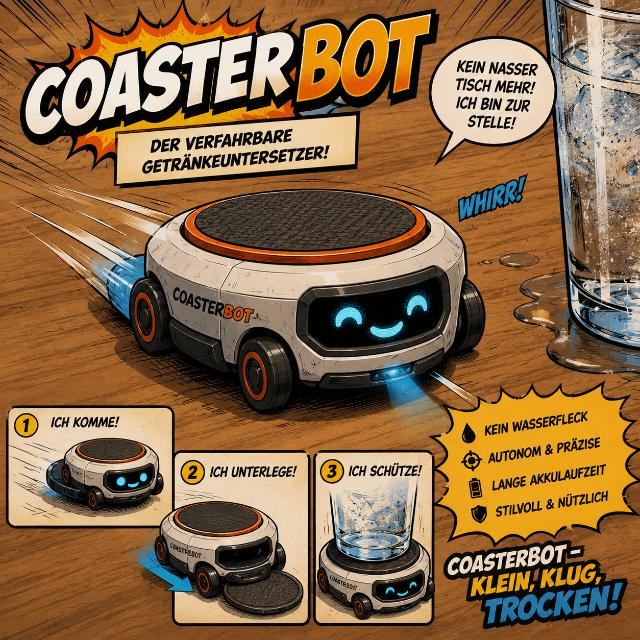
\includegraphics[width=0.38\textwidth]{coasterbot.png}} \\[1em]

\vspace{4em}

    {\normalsize
\begin{tabular}{ll}
Dennis Borutta, B. Eng & dennis.borutta@outlook.com\\
Stefan Etringer, B. Eng & mail@stefan.works\\
Gereon Such, M. Sc. & gereonsuch@gmail.com\\
\end{tabular}
    }
  \end{center}


\end{titlepage}


% einleitung preambel etc.


% Versionshistorie des Dokuments -- eigene Seite direkt nach dem Titelblatt
\section*{Versionshistorie}

\begin{tabularx}{\textwidth}{@{}clp{2.6cm}X@{}}
\toprule
\textbf{Version} & \textbf{Datum} & \textbf{Bearbeiter} & \textbf{Änderungen}\\
\midrule
1 & 24.08.2026 & Borutta & Erstfassung der Konzeptbeschreibung\\
2 & 18.10.2026 & Borutta & Finalisierung \\
\bottomrule
\end{tabularx}


\newpage

\tableofcontents

\newpage

\section{Konzeptbeschreibung}\label{coasterbot-konzeptbeschreibung}

\subsection{Übersicht}\label{uebersicht}

Der Coasterbot ist ein mobiler Roboter auf einem vierrädrigen Chassis,
dessen zentrale Funktion die \textbf{Aufnahme und Ausgabe von
Untersetzern} ist. Der Roboter ist mit einem Lochraster-Chassis
aufgebaut, das eine flexible Montage von Elektronik, Sensorik und
Mechanik erlaubt. Aus diesem Grund sind in den folgenden Bildern noch
nicht alle Komponenten sichtbar. Deren ideale Platzierung kann am
Prototyp variieren und so der optimale Platz gefunden werden. Vier
einzeln angetriebene Räder sorgen für die Fortbewegung, während im
Zentrum des Fahrzeugs ein Mechanismus zur Untersetzerhandhabung
untergebracht ist.

\subsection{Gesamtkonzept}\label{gesamtkonzept}

Die folgenden Ansichten zeigen das grundlegende Layout des Roboters
aus der Vogelperspektive sowie von vorne.

\subsubsection{Draufsicht (Konzept)}\label{draufsicht-konzept}

\begin{figure}
\centering
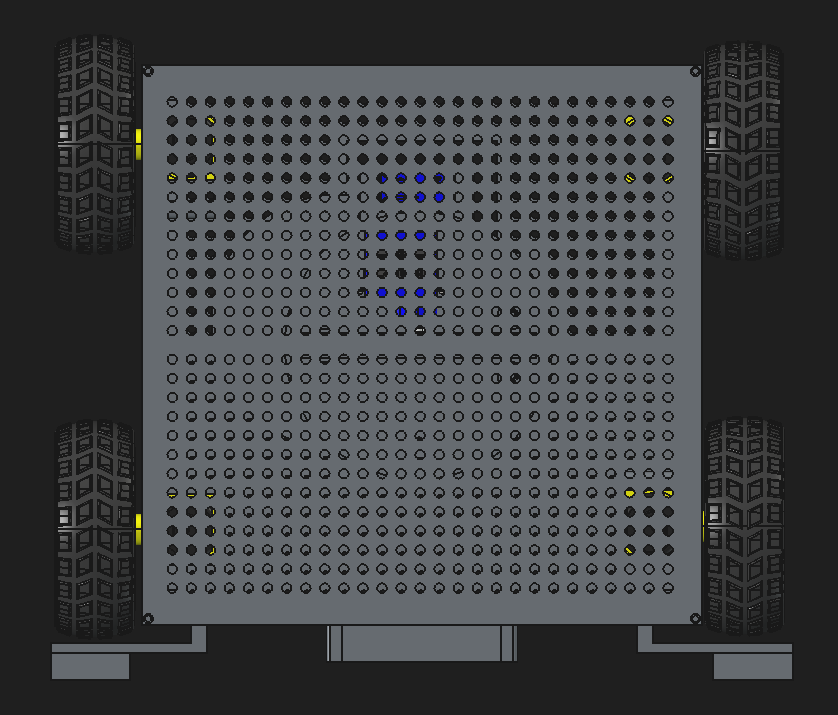
\includegraphics[width=0.75\textwidth,keepaspectratio,alt={Konzept Draufsicht}]{Konzept_Draufsicht.png}
\caption{Konzept Draufsicht}
\label{draufsicht-konzept}
\end{figure}

Die Draufsicht in Abbildung~\ref{draufsicht-konzept} zeigt die symmetrische Anordnung der vier Räder in den
Ecken des Chassis. Die blau durchscheinende Bereiche kennzeichnen die
Position der Servomotoren für die Ausgabe und Aufnahme von Untersetzer,
die gelb durchscheinenden Bereiche sind die verwendeten Antriebsmotoren
zur Fortbewegung. Befestigt wird die obere Platte über vier Schrauben an
das Grundgestell. Damit Klemmt diese obere Platte vier Seitenwände in
das Grundgestell ein.

\subsubsection{Frontansicht (Konzept)}\label{chapter_frontansicht-konzept}

\begin{figure}
\centering
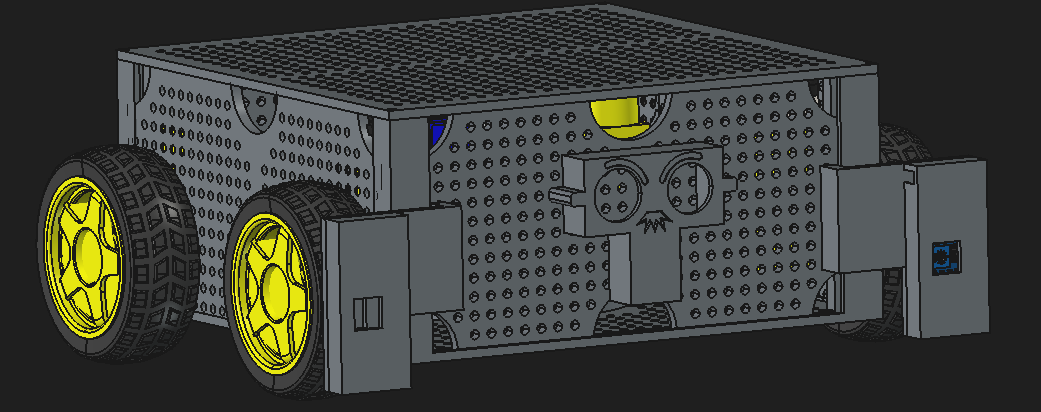
\includegraphics[width=0.75\textwidth,keepaspectratio,alt={Konzept schräge Frontansicht}]{Konzept_Frontansicht.png}
\caption{Konzept schräge Frontansicht}\label{frontansicht-konzept}
\end{figure}

Die Frontansicht in Abbildung~\ref{frontansicht-konzept} verdeutlicht das Fahrzeug sowie die Anbringung der
Sensoren zur Kanten- und Hinderniserkennung. Mittig ist eine stilisierte
„Gesichts''-Blende zu erkennen, welche einen Ultraschallsensor aufnimmt. Dieser wird zur Hinderniserkennung verwendet. Die vor den Rädern stehenden Gehäuse sind zur Aufnahme der Sensorik zur Kantenerkennung gedacht. Diese sind auch für die hinteren Räder vorgesehen. Die Antriebsräder werden über einen Halter mit den Außenwänden verschraubt. Alle Außenwände werden von oben in das Grundgestell eingeschoben. Ein Fixierung der Wände erfolgt über die Führungen in den Eckpfeilern, dem Deckel und der Grundplatte.

\subsection{Mechanischer Aufbau}\label{mechanischer-aufbau}

\subsubsection{Isometrische Ansicht ohne
Deckel}

\begin{figure}
\centering
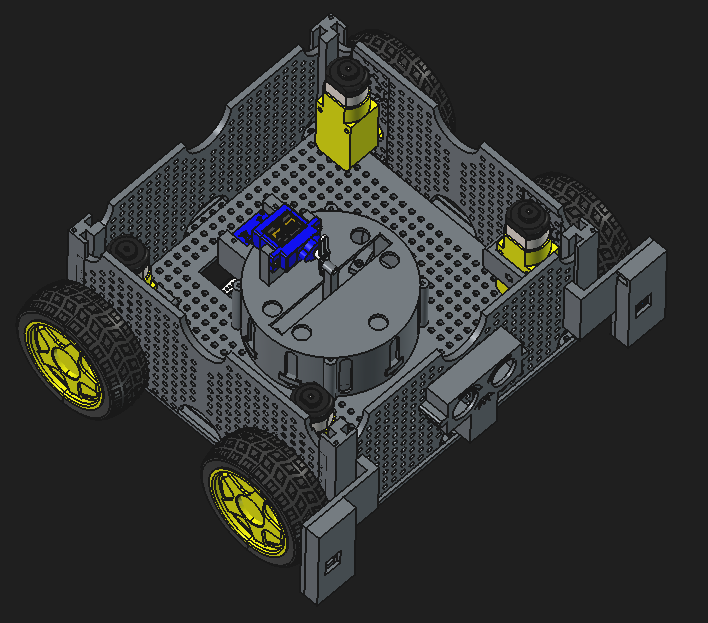
\includegraphics[width=0.75\textwidth,keepaspectratio,alt={Coasterbot Isometrische Ansicht ohne Deckel}]{Coasterbot_Iso_Draufsicht_ohne_Deckel.png}
\caption{Coasterbot Isometrische Ansicht ohne Deckel}\label{isometrische-ansicht-ohne-deckel}
\end{figure}

Die Darstellung in Abbildung~\ref{isometrische-ansicht-ohne-deckel} zeigt den Innenaufbau des Roboters ohne die obere Abdeckung. Im Zentrum ist die Untersetzermechanik zur Aufnahme und Ausgabe der Untersetzer zu erkennen. Sie besteht aus einem Gehäuse, einem beweglichen Stempel mit mehreren eingelassenen Magneten, Verbindungsstücken, einem Auswurf-/Führungssteg und zwei Servo-Motoren. Es wird ein Schubkurbeltrieb verwendet um den Stempel auf und ab zu bewegen. Der Antrieb erfolgt über den oberen Servomotor. Durch die im Stempel befindlichen Magneten werden speziell gefertigte Untersetzer angezogen und aufgenommen. Es wird ausreichend Platz vorgesehen, dass wenigsten vier Untersetzer in dieser Mechanik vorgehalten werden. 

An den vier Ecken des Chassis sind die Antriebsmotoren der Räder zu sehen. Bei dem rechts im Bild befindlichen Antriebsmotor ist dier Halter zur Befestigung eingeblendet. Mit diesem Halter werden alle weiteren Antriebsmotoren ebenfalls befestigt.

\subsubsection{Untere Ansicht}\label{chapter_untere-ansicht}

\begin{figure}
\centering
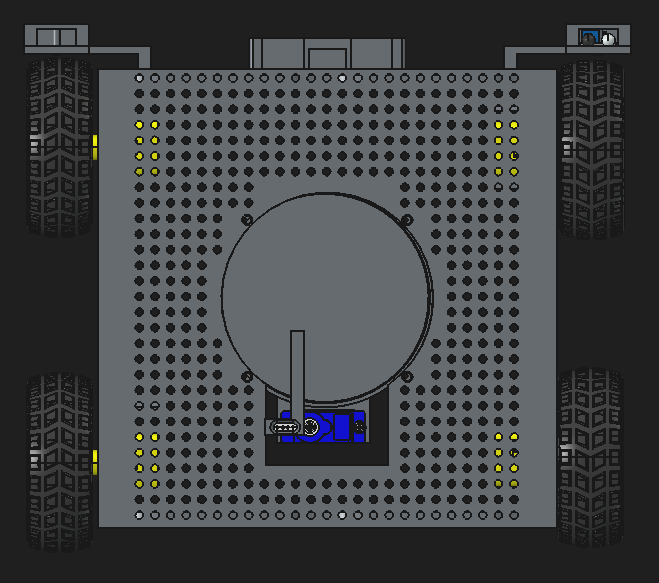
\includegraphics[width=0.75\textwidth,keepaspectratio,alt={Coasterbot untere Ansicht}]{Coasterbot_untere_Ansicht.png}
\caption{Coasterbot untere Ansicht}
\label{untere-ansicht}
\end{figure}

In Abbildung~\ref{untere-ansicht} ist zentral die Unterseite der Untersetzermechanik mit dem herausragenden Auswurf-/Führungssteg sowie dem zweiten Servomotor erkennber. Wird ein Untersetzer ausgegeben, wird dieser soweit heruntergelassen, dass er auf dem Führungssteg abliegt. Anschließen rotiert der Servomotor um 90° wodurch die kurze Seite des Auswurf-/Führungssteg den Untersetzer nach vorne schiebt. Durch ein anschließendes Anheben des Hebemechanismus, wird der Untersetze abgelegt. Wird ein Untersetzer wieder aufgenommen, dreht sich der Ausschieber weitere 90° zur Seite, damit der Stempel an der Mechanik vorbeikommt. Dadurch kann der Stempel soweit heruntergefahren werden, bis die Magneten den sich darunter befindlichen Untersetzer anziehen und damit aufnehmen. Befestigt wird die Mechanik mit dem Gehäuse über vier Schrauben.

\subsubsection{Spätere Nacharbeit}
Im Laufe des Projekts stellte sich heraus, dass es Nachbesserungbedarf im mechanischen Konzept. Diese sind hier gelistet:
\begin{enumerate}
  \item Erneuerung der Halter zur Motoraufnahme, damit ein Encoder montiert werden kann
  \item Entfernen der Führungsstücke am Stempel der Untersetzermechanik
  \item Anpassen des Auswurf-/Führungssteg für einen stärkeren Servomotor und vergößern der Auflagefläche am Führungssteg für Untersetzer
\end{enumerate}

\newpage
\section{Anhang}
\subsection{Zeichnungen Coasterbot}
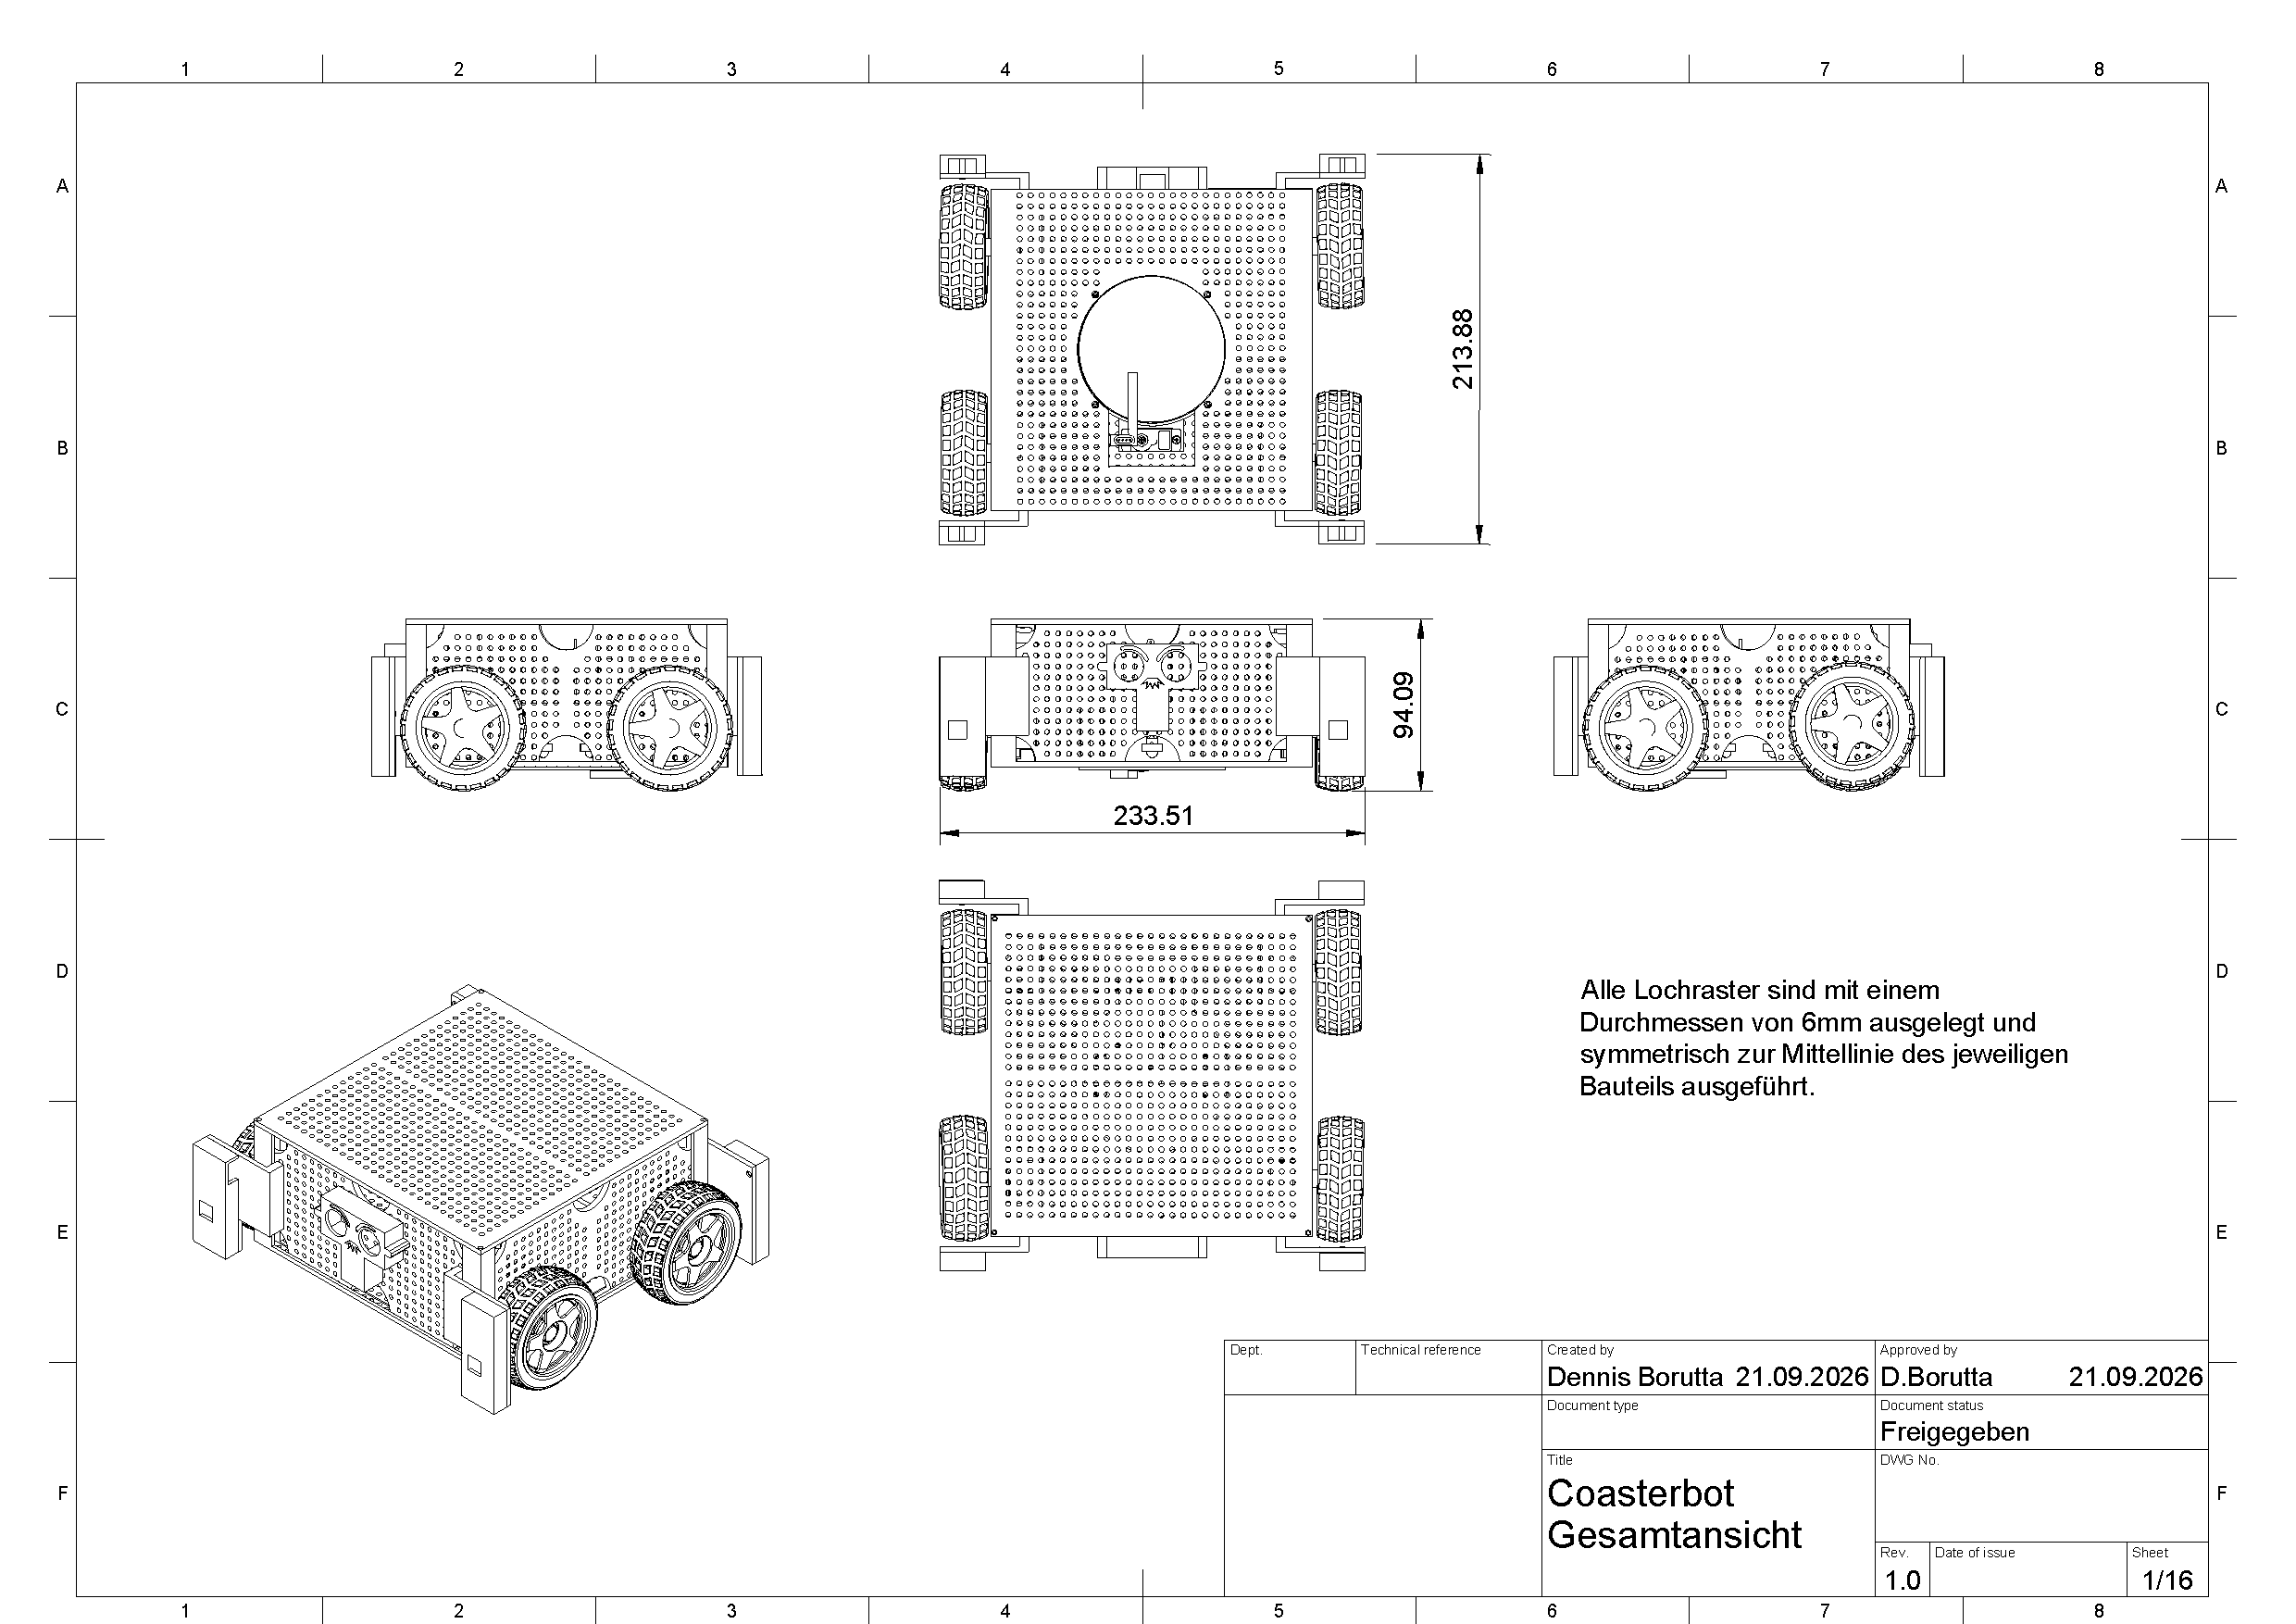
\includepdf[pages=-,landscape=true]{Technische Zeichnungen/Coasterbot.pdf}

\subsection{Zeichnung Untersetzer}
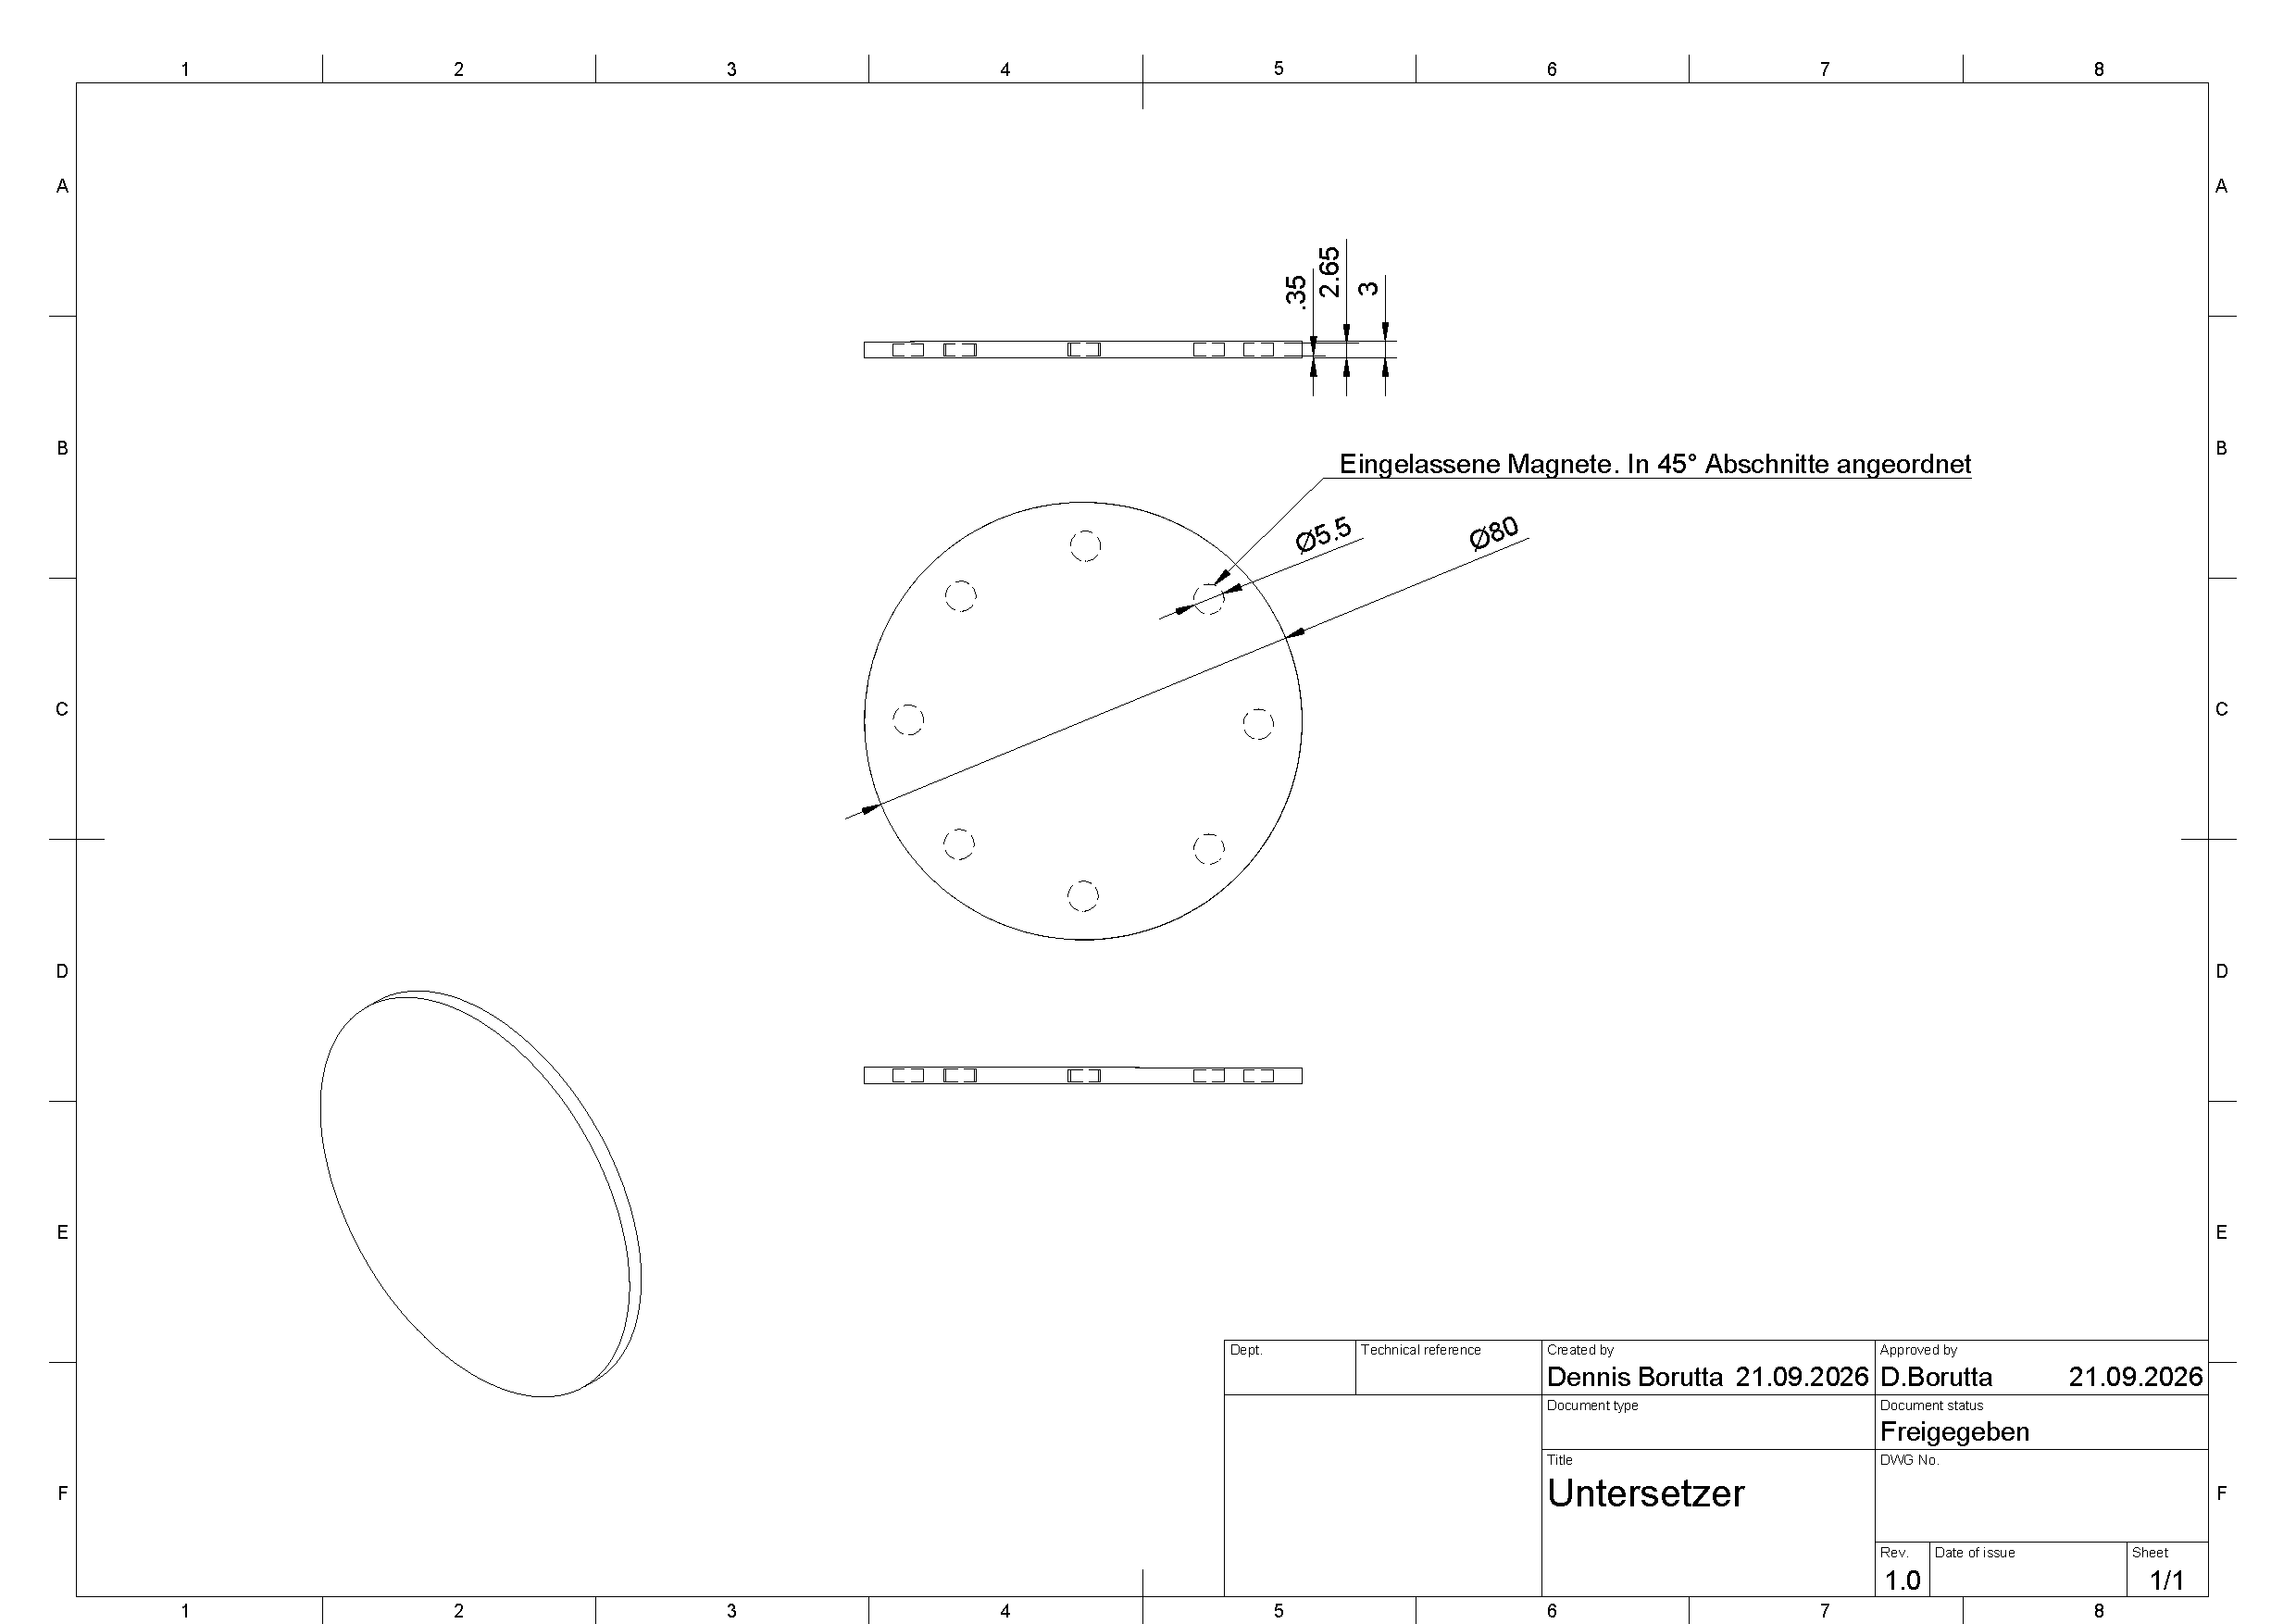
\includepdf[pages=-,landscape=true]{Technische Zeichnungen/Untersetzer.pdf}

\subsection{Zeichnung Nacharbeit}
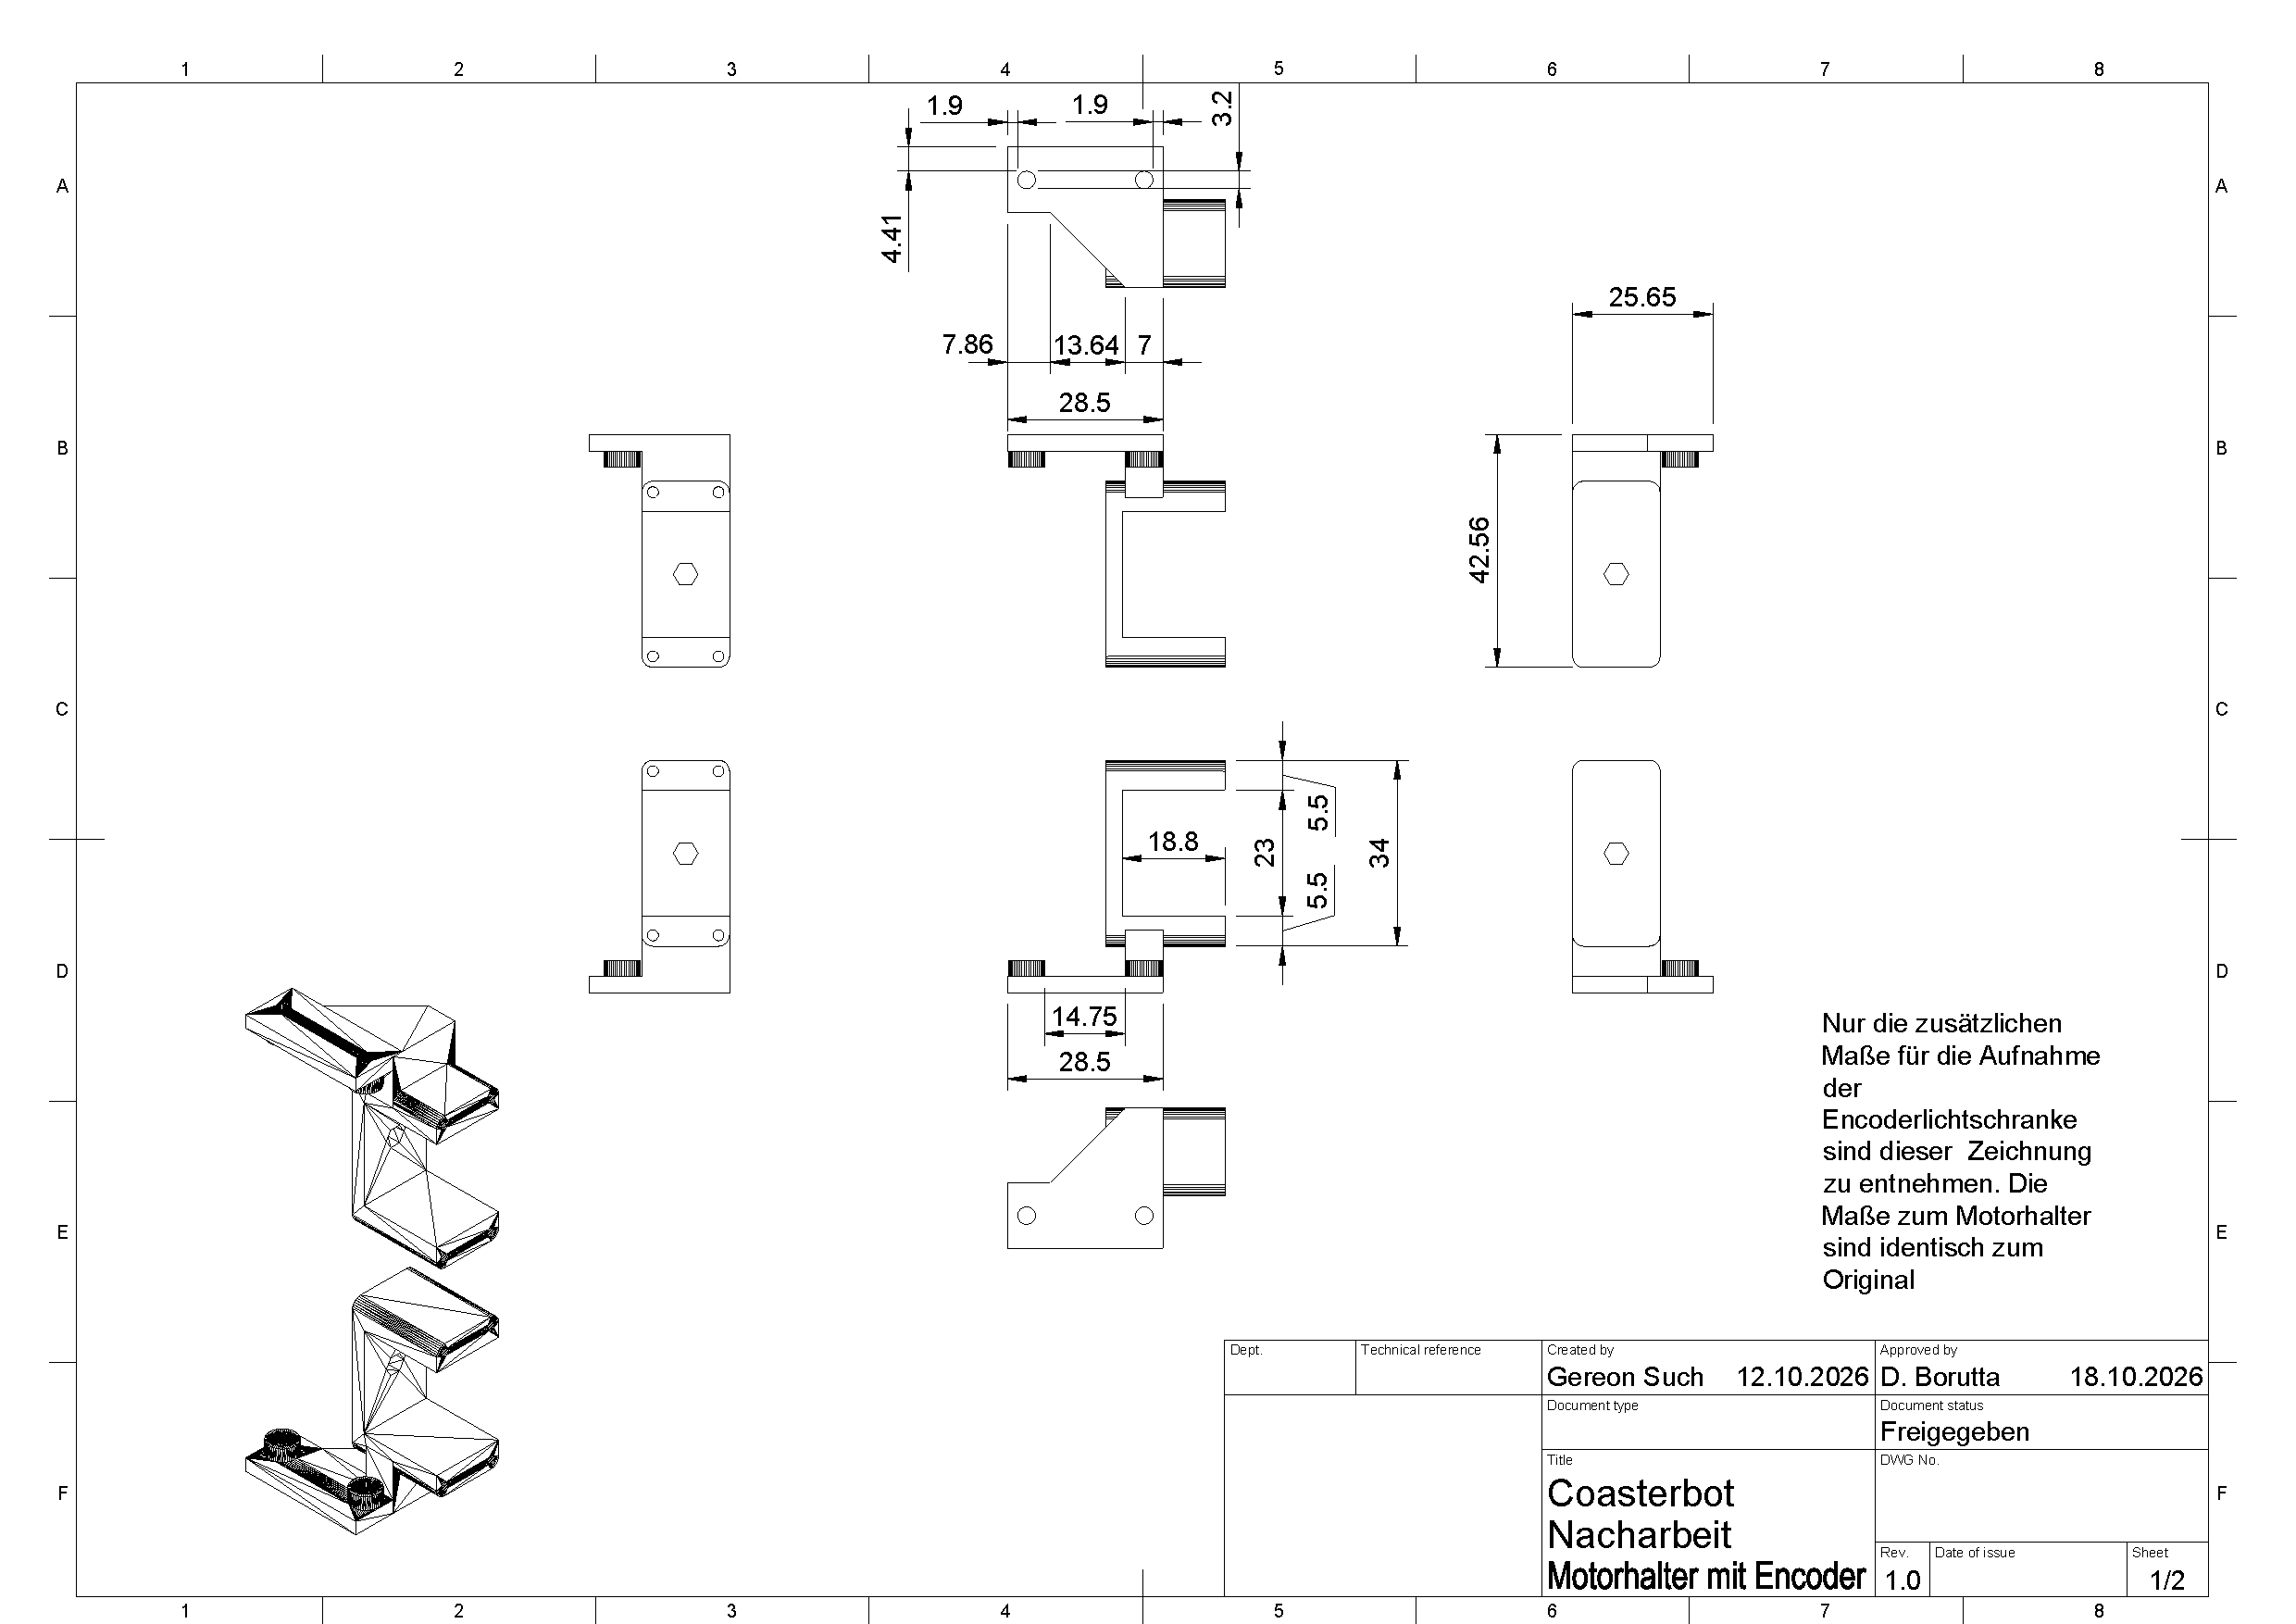
\includepdf[pages=-,landscape=true]{Technische Zeichnungen/Nacharbeit.pdf}



\end{document}
